\documentclass[a4wide]{article}
\usepackage{a4wide}
\usepackage{appendix}
\newcommand{\comment}[1]{{\tt #1}}
\usepackage{graphicx}

\title{HurdleJumpr:\\ OO Software System Design}

\author{Hesham H. Salman \and Jonathon Kissinger \and Sean Mead \and Troy Johnson}

\begin{document}
\maketitle

\section{External Design Specifications}
The design for layout for the user game will be relatively simple. When the user launches the game, they will be presented with the menu in FIGURE 1.
\begin{figure 1}
    \centering
    \textbf{Figure 1}\par\medskip
    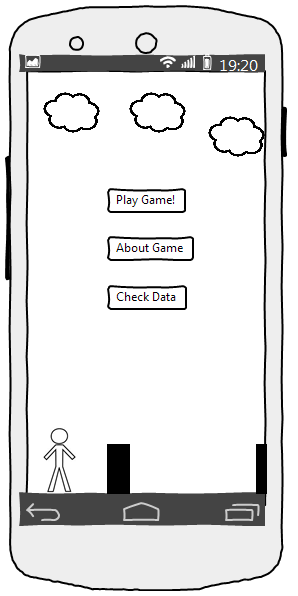
\includegraphics[height=8cm]{images/intro.png}
    \caption{Figure 1}
\end{figure 1}

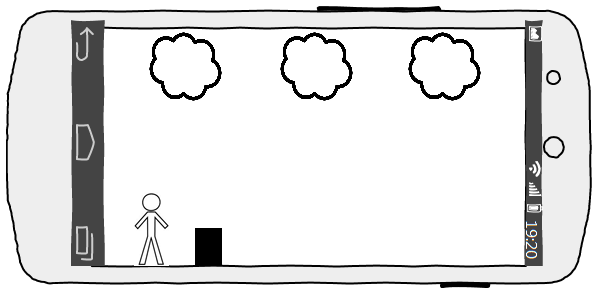
\includegraphics[width =8cm,height=5cm]{images/screen_layout.png}
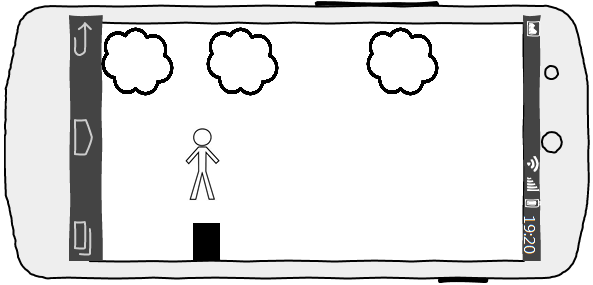
\includegraphics[width =10cm,height=5cm]{images/user_jumping.png}
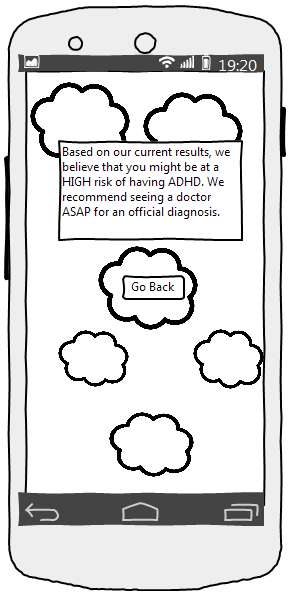
\includegraphics[height=8cm]{images/diagnosis_screen.png} The user will have the option play the game, view details about the makers of the game, of check the results of their data was most recently sent in for processing. If the user selects to play the game they will be presented with a layout similar to FIGURE 2. FIGURE 2 is the basic game, more details may be added later if time permits. The design will be a side scroller game with the user being represented by a character of some sort (a stick figure in FIGURE 2. The user will then have to jump over the black blocks that show up as show in FIGURE 2 as the characters moves from left to right across the screen.  A figure of the user jumping can be seen in FIGURE 3. Once the user has finished playing, their reactions time are uploaded and once their results are received the user will see a screen similar to that of FIGURE 4, where they are notified about their results. The results of our mining of their response time data may become more detailed later on depending upon how accurate we can get with out predictions.
\section{Architectural Design Specifications}
%%%%%%%%%%%%%%%%%%%%%%%%%%%%%%%%%%%%%%%%%%%%%%%%%%%%%%%%%%%%%%%%
\section{Detailed Design Specifications}

\subsection{Interface Specifications}

\subsection{Class Definitions}

\subsection{Algorithms}

\subsection{Data file specifications}


%%%%%%%%%%%%%%%%%%%%%%%%%%%%%%%%%%%%%%%%%%%%%%%%%%%%%%%%%%%%%%%%
\section{Test Plan}
\begin{enumerate}
\item Performance tests
\begin{enumerate}


\item a.	User interface
\begin{enumerate}
\item	Ease of use - Ask those unfamiliar with the project, and no more than a beginner’s knowledge of the game to attempt to play the game. Ask user on how they think the game could be improved or what may have confused them.
\item	Ease of use on touch device – Make sure icons work fine on touch devices, i.e, make sure that all click-able icons that are used aren't so small that a user with rather large fingers would have trouble playing
\item	Compatibility with other Android operating system versions – Mobile game application should be compatible with at least Android Jelly Bean (Android 4.0) or higher. This means that the mobile game will have to be tested on mobile devices with Android Jelly Bean, Android Kit Kat, and possibly Android L (if released in time).
\item 	Other design goals as needed (as more detail is added to the SRS)
\end{enumerate}
\item	Overall system
\begin{enumerate}
\item	 Response time should be quick. No more than 1 second without feedback to the user on their results. Wait times that are required to be longer than that should show a dialog giving an estimated wait time if possible, and a general spinner waiting dialog if not  to show that the app is retrieving or uploading data (Source: http://www.useit.com/papers/responsetime.html)
\item	Availability – System should always be available other than when maintenance is being performed on the server. Test what happens if the system is shut down while a client is actively playing the game and/or uploading the results of their game. Other than when the server/system is down for maintenance, the system should always be up and running and therefore a user playing the game at any time should be able to upload the data from their game at almost any time.
\item	Security - Normal security measures; to test this we could possibly invite a person with hacking knowledge to attempt to hack the system. Also, gather advice on the security aspects from the security professionals  and ask them what we could do to increase the security of the system.
\item	Recovery - How does the system respond if the client’s connection is lost when uploading the user’s data to the server?
v.	Other design goals as needed (as more detail is added to the SRS)
\end{enumerate}

\item	Stress tests
\begin{enumerate}
\item	Manual - A test where 10 (hopefully more depending on how many testers we can get) logged-in users perform the same functions and see if any wait times or ramp up times occur. This test will help determine how the server reacts to periods of time where many people may be submitting their response time data to the server at the same time for processing.
\item	Automatic – Set up a testing scenario with some open source software testing tool that can simulate as many simultaneous connections as needed (hundreds? thousands?), similar to an integration test. This can method can also be used to determine the maximum number of concurrent users that the server can support under a given configuration.
\item	Automatic (Similar style as mentioned in b) – Perform a long-running stress test that drives a continuous load on the server for an extended period of time.  (Due to time constraints “long-running” may only consist of a week at most) The main purpose of this type of test would be to ensure the server accepting the data can sustain acceptable levels of performance over an extended period of time without exhibiting any slowdowns.
\item	User monkeyrunner to simulate thousands of pseudorandom presses in places on the game and see if the application breaks.
\end{enumerate}
\end{enumerate}
3.	Functional tests
\begin{enumerate}
\item	Specific test cases:
\begin{enumerate}
\item	User submits response time data with no connection to the server currently available
\item	User loses connection in the middle of uploading their data to the server
\item	User uploads their same data to the server multiple times
\item	User is the first to submit their data to the server (no data to compare against to help determine ADHD diagnosis)
\item	User quits in the middle of the game, make sure data isn’t submitted.
\item	User doesn’t give permission to upload their information

\end{enumerate}
\end{enumerate}

\section{References}
\section{Appendices}
\end{document}